\documentclass[11pt]{article}
\usepackage{amssymb}
\usepackage{amsthm}
\usepackage{enumitem}
\usepackage{physics,amsmath}
\usepackage{bm}
\usepackage{adjustbox}
\usepackage{mathrsfs}
\usepackage{graphicx}
\usepackage{siunitx}
\usepackage[mathscr]{euscript}

\title{\textbf{Solved selected problems of Classical Mechanics - Gregory}}
\author{Franco Zacco}
\date{}

\addtolength{\topmargin}{-3cm}
\addtolength{\textheight}{3cm}

\newcommand{\hatr}{\bm{\hat{r}}}
\newcommand{\hatx}{\bm{\hat{x}}}
\newcommand{\haty}{\bm{\hat{y}}}
\newcommand{\hatz}{\bm{\hat{z}}}
\newcommand{\hatn}{\bm{\hat{n}}}
\newcommand{\hati}{\bm{\hat{i}}}
\newcommand{\hatj}{\bm{\hat{j}}}
\newcommand{\hatk}{\bm{\hat{k}}}
\newcommand{\hatth}{\bm{\hat{\theta}}}
\newcommand{\hatphi}{\bm{\hat{\phi}}}
\newcommand{\hatrho}{\bm{\hat{\rho}}}
\newcommand{\ngrad}[1]{\text{grad}_{\bm{#1}}}

\theoremstyle{definition}
\newtheorem*{solution*}{Solution}
\renewcommand*{\proofname}{\bf{Solution}}

\begin{document}
\maketitle
\thispagestyle{empty}

\section*{Chapter 16 - Vector angular velocity and rigid body kinematics}

\begin{proof}{\textbf{16.1}}
    The vector $\hatn$ in this case points in the positive $z$ direction
    i.e. $\hatn = \hatk$ then the angular velocity vector is given by
    \begin{align*}
        \bm{\omega} = 2\hatk~~\text{radians per second}
    \end{align*}
    To determine the instantaneous velocity of $P = (4, -3 ,7)$
    we first write that $\bm{r} = 4\hati + -3\hatj + 7\hatk$ and hence
    \begin{align*}
        \bm{v} &= (2\hatk) \times (4\hati + -3\hatj + 7\hatk)\\
            &= \begin{vmatrix}
                \hati & \hatj & \hatk\\
                0 & 0 & 2\\
                4 & -3 & 7
            \end{vmatrix}\\
            &=  6\hati + 8\hatj~m/s
    \end{align*}
    The speed is therefore $|\bm{v}| = \sqrt{6^2 + 8^2} = 10~m/s$
    Finally, the acceleration of $P$ can be found using that
    $\bm{a} = \bm{\omega} \times \bm{\dot{r}}$ hence
    \begin{align*}
        \bm{a} &= \bm{\omega} \times \bm{v}\\
            &= (2\hatk) \times (6\hati + 8\hatj)\\
            &= \begin{vmatrix}
                \hati & \hatj & \hatk\\
                0 & 0 & 2\\
                6 & 8 & 0
            \end{vmatrix}\\
            &= -16\hati + 12\hatj~m/s^2
    \end{align*}
\end{proof}
\cleardoublepage
\begin{proof}{\textbf{16.3}}
    In this case, the system looks like the following
    \begin{center}
        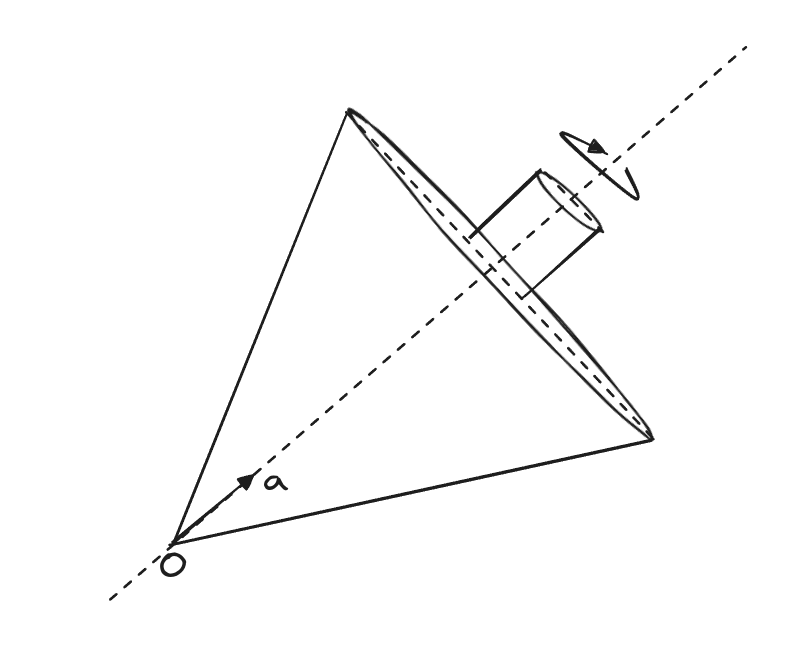
\includegraphics[scale=0.35]{ch16-3.png}
    \end{center}
    We know that the particle at the origin is fixed so Theorem 16.1 
    applies and hence the velocity of any particle of the spinning top
    is given by
    \begin{align*}
        \bm{v} = \bm{\omega} \times \bm{r}
    \end{align*}
    In particular, this must be true for any particle lying on the axis of 
    symmetry. These particles have a position vector given by $\beta\bm{a}$
    where $\beta$ is a scalar and $\bm{a}$ is the unit vector pointing along
    the axis of symmetry, hence we have that 
    \begin{align*}
        \beta\bm{\dot{a}} &= \bm{\omega} \times (\beta\bm{a})
    \end{align*}
    Which implies that
    \begin{align*}
        \bm{\dot{a}} = \bm{\omega} \times \bm{a}
    \end{align*}
    On taking the cross product of this equation with $\bm{a}$, we obtain
    \begin{align*}
        \bm{a} \times \bm{\dot{a}} 
        &= \bm{a} \times (\bm{\omega} \times \bm{a})\\
        &= (\bm{a} \cdot \bm{a})\bm{\omega} - (\bm{a} \cdot \bm{\omega})\bm{a}
    \end{align*}
    Since $\bm{a}$ is a unit vector we have that $\bm{a} \cdot \bm{a} = 1$
    and hence 
    \begin{align*}
        \bm{\omega}
        &= \bm{a} \times \bm{\dot{a}} + (\bm{a} \cdot \bm{\omega})\bm{a}
    \end{align*}    
    It follows that $\bm{\omega}$ must have the following form
    \begin{align*}
        \bm{\omega}
        &= \bm{a} \times \bm{\dot{a}} + \lambda\bm{a}
    \end{align*}
    Where $\lambda$ is a scalar function of the time.
\end{proof}
\cleardoublepage
\begin{proof}{\textbf{16.4}}
    In this case, we are considering a system that looks like the following
    \begin{center}
        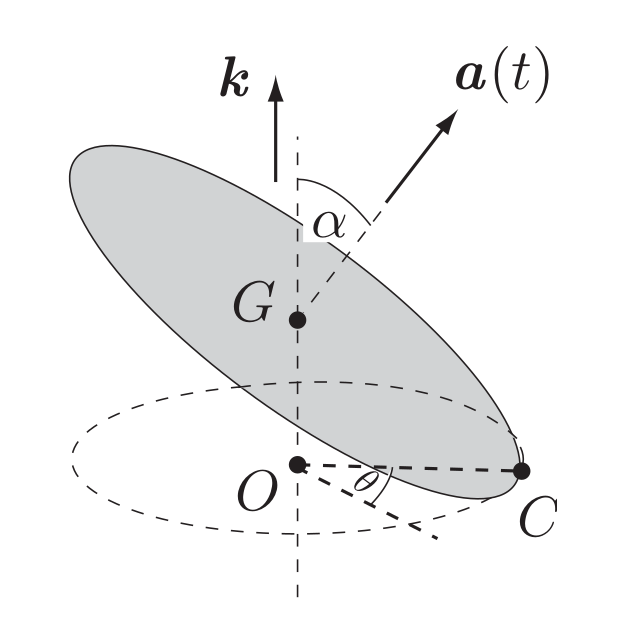
\includegraphics[scale=0.4]{ch16-4.png}
    \end{center}
    Suppose we view the motion of the penny about a rotating reference frame
    with respect to the $\hatk$ axis, then the angular velocity $\bm{\Omega}$
    of the frame is given by
    \begin{align*}
        \bm{\Omega} = \dot{\theta}\hatk
    \end{align*}
    From this rotating reference frame, the axis $\bm{\hat{a}}$
    is fixed so the penny rotates about $\bm{\hat{a}}$ with an angular velocity
    \begin{align*}
        \bm{\omega'} = \lambda\bm{\hat{a}}
    \end{align*}
    for some function $\lambda$.
    Then using the result of the angular velocity addition theorem,
    stated in Chapter 17, we get that 
    \begin{align*}
        \bm{\omega} &= \bm{\Omega} + \bm{\omega'}\\
        &= \dot{\theta}\hatk + \lambda\bm{\hat{a}}
    \end{align*}
    So by taking the dot product of the equation with $\bm{\hat{a}}$
    we have that
    \begin{align*}
        \bm{\omega} \cdot \bm{\hat{a}}
        &= \dot{\theta}\hatk\cdot \bm{\hat{a}}
        + \lambda\bm{\hat{a}} \cdot \bm{\hat{a}}
        = \dot{\theta}\cos\alpha + \lambda
    \end{align*}
    Instantaneously the point $C$ because of the rolling condition is fixed
    but also $G$ is fixed then $\bm\omega$ must be perpendicular to
    $\bm{\hat{a}}$ and hence
    \begin{align*}
        \dot{\theta}\cos\alpha + \lambda &= 0\\
        \lambda &= -\dot{\theta}\cos\alpha
    \end{align*}
    Therefore $\bm\omega = \dot{\theta}(\hatk - \cos\alpha \bm{\hat{a}})$.

    Finally, from particle $G$ (which is fixed) the velocity of the highest
    particle is given by $\bm{v} = \bm\omega \times \bm{r}$
    but the vector $\bm{r}$ instantaneously from what we saw earlier
    is in the same direction as $\bm\omega$ therefore
    $\bm{v} = 0$ for the highest particle.
\end{proof}
\begin{proof}{\textbf{16.5}}
    In this case, we are considering a system that looks like the following
    \begin{center}
        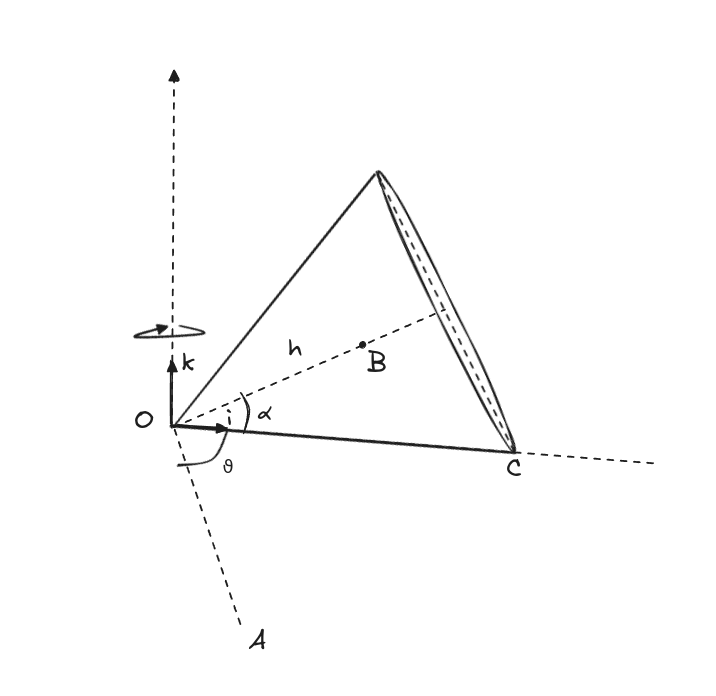
\includegraphics[scale=0.4]{ch16-5.png}
    \end{center}
    First, because the cone rolls without slipping we know that every point in
    the line $OC$ (the line in contact with the table) must have $v = 0$ this
    includes the vertex $O$ of the cone so it never moves.

    Let us consider now a particle in the line $OC$ then given that the point
    $O$ is fixed then the particle has a velocity given by
    $\bm{v} = \bm{\omega} \times d\bm{i}$ where $d$ is the distance from $O$ 
    to the particle and $\bm{i}$ is the unit vector in the $OC$ direction.
    But we know that particles in the $OC$ line have $\bm{v} = 0$
    so we get that $\bm{\omega} \times d\bm{i} = 0$ which implies that
    $\bm\omega$ is parallel to $\bm i$ hence we can write $\bm\omega$ as
    $\bm\omega = \lambda \bm{i}$ for some function $\lambda$.

    On the other hand, let us consider a particle in the axis of symmetry
    at some point $B$ at a distance $r$ from the origin $O$ then
    this particle has a velocity of 
    \begin{align*}
        \bm{v} &= \bm{\omega} \times \bm{r}\\
            &= \lambda \bm{i} \times (r\sin\alpha\bm{k} + r\cos\alpha \bm{i})\\
            &= \lambda \bm{i} \times r\sin\alpha\bm{k}\\
            &= \lambda r\sin \alpha~(\bm{i} \times \bm{k})
    \end{align*}
    Where $\bm{k}$ is the unit vector pointing in the $z$ direction as shown.
    Also, we could see the particle $B$ as a particle rotating around the $z$
    axis with a velocity of magnitude $v = -\dot\theta (r\cos\alpha)$ where 
    we take a minus sign since the angle $\theta$ is decreasing so by
    joining these results we get that
    \begin{align*}
        \lambda r\sin \alpha &= -\dot\theta r\cos\alpha\\
        \lambda &= -\dot\theta \frac{\cos\alpha}{\sin \alpha}\\
        \lambda &= -\dot\theta \cot\alpha
    \end{align*}
    Therefore the angular velocity is given by
    \begin{align*}
        \bm\omega = -(\dot\theta \cot\alpha) \bm{i}
    \end{align*}
    Finally, from what we saw the particle with the maximum speed will be the
    one the furthest perpendicularly from the $OC$ axis.
    From trigonometry, we know that $OC = h/\cos\alpha$ then the furthest point
    perpendicularly is at a distance
    $$OC \sin 2\alpha = \frac{h\sin 2\alpha}{\cos\alpha}
    = \frac{2h\sin\alpha\cos\alpha}{\cos\alpha} = 2h\sin\alpha$$
    Therefore the speed of this point is 
    \begin{align*}
        |v| = 2h|\dot\theta| \cot\alpha \sin\alpha = 2h|\dot\theta|\cos\alpha
    \end{align*}
\end{proof}









\end{document}



















